\section{Mise en place d'une solution \alinotp{}}

\subsection{Principe des \etranger{One-Time Passwords} (OTP)}

\paragraph{}
Les \etranger{One-Time Passwords}, aussi appelés OTP, sont des mots de passe générés à un instant donné, valides pendant une courte durée et utilisables une seule fois.
La génération s'effectue grâce à des matériels adaptés, comme les tokens (\cffigure{linotp:token}) ou même des smartphones.

\begin{figure}
	\centering
	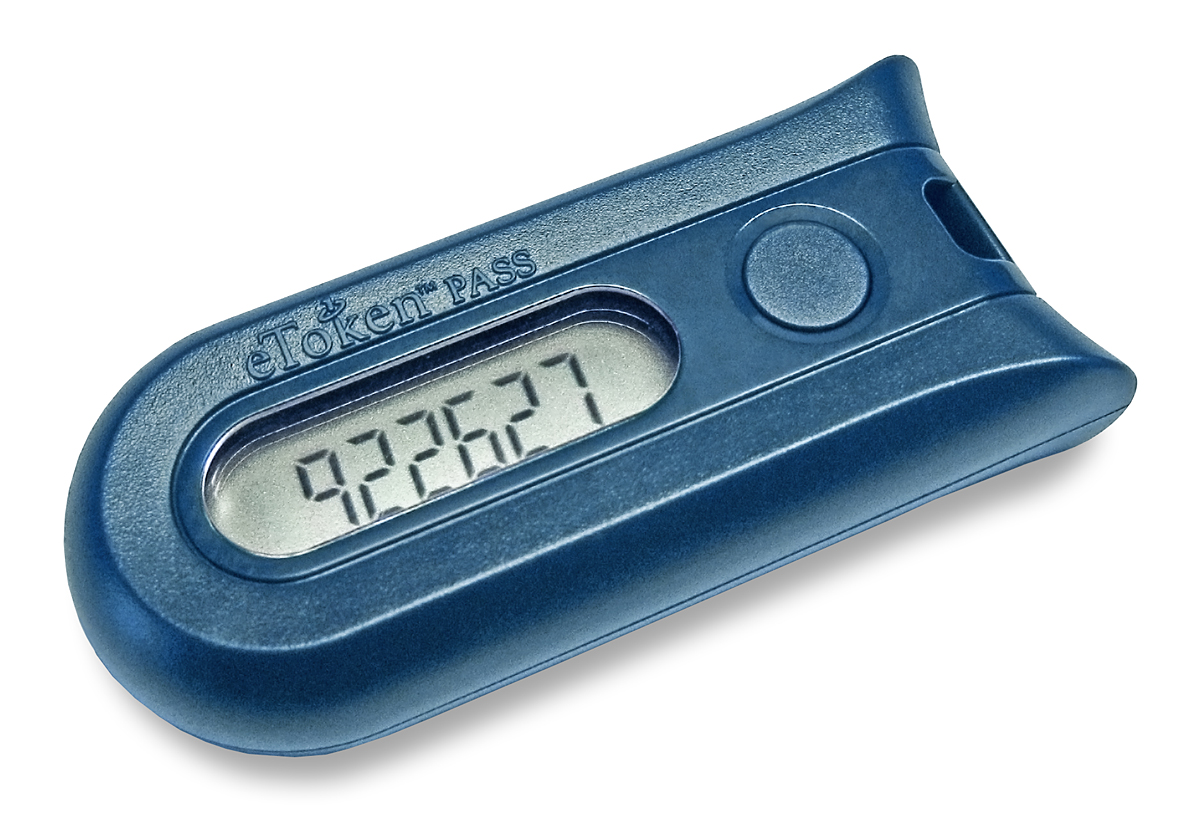
\includegraphics[width=6cm]{linotp/etoken_pass}
	\caption{Token Aladdin eToken-PASS}
	\label{figure:linotp:token}
\end{figure}

\paragraph{}
En pratique, l'utilisateur final s'authentifie en précisant son identifiant, son PIN -- qui correspond à un mot de passe statique qu'il doit mémoriser -- et l'OTP obtenu grâce au matériel.
C'est en ce sens qu'on peut parler de système à deux facteurs d'authentification (\etranger{two-factor authentication}) car on se base sur quelque chose que l'on connaît -- le PIN -- et quelque chose que l'on possède -- le token ou le smartphone.

\paragraph{}
Ainsi, l'OTP permet de résoudre un certain nombre de problèmes inhérents à l'utilisation de mots de passe statiques classiques :

\begin{itemize}
	\item on n'est plus soumis aux limites du facteur humain, qui implique souvent des compromis sur la complexité du mot de passe, et l'irrégularité de son changement ;
	\item en particulier les attaques par dictionnaire deviennent inefficaces ;
	\item les attaques par brute-force sont également limitées car elles ne peuvent plus se baser que sur des essais aléatoires dans un grand espace de clés ;
	\item la récupération silencieuse du mot de passe (via l'écoute réseau, l'installation d'un mouchard, ou l'ingénierie sociale) ne suffit plus à s'authentifier.
\end{itemize}

\paragraph{}
Par ailleurs, une méthode de génération d'OTP se base sur la synchronisation temporelle : les tokens et le serveur d'authentification OTP sont réglés à la même heure.
De plus, pour chaque token est définie une clé secrète que l'on enregistre dans la base du serveur.
C'est la combinaison de ces deux paramètres qui permet une génération et une validation des OTP.


\subsection{Contexte de la mission}

\paragraph{}
Au courant de l'année 2010, la Commission nationale de l'informatique et des libertés\footnote{La CNIL est une autorité administrative indépendante française.Elle est chargée de veiller à ce que l'informatique soit au service du citoyen et qu'elle ne porte atteinte ni à l'identité humaine, ni aux droits de l'homme, ni à la vie privée, ni aux libertés individuelles ou publiques.\cite{cnil}} (CNIL) décide d'ouvrir son portail \aintranet{} pour certains de ses utilisateurs : les commissaires.
Au nombre d'une vingtaine, ceux-ci ont besoin d'accéder au contenu du site web à l'extérieur de leur lieu de travail, à la maison par exemple.

\paragraph{}
La CNIL avait déjà fait appel aux prestations de \asmile{} pour bénéficier d'un support ponctuel sur des développements \atypo{}, le système de gestion de contenu utilisé pour le portail.
C'est pour cela qu'elle a également choisi \asmile{} pour mettre en place l'architecture permettant un tel accès depuis l'extérieur.

\paragraph{}
C'est la CNIL elle-même qui a choisi le type d'autentification à utiliser : les OTP.
\asmile{} a alors proposé fin 2010 l'utilisation d'une solution de la marque RSA, leader sur ce marché.
Pour des raisons qui sont restées inconnues -- le nombre de licences commandées était trop faible ? -- RSA n'a pas daigné répondre aux commandes de licences et de matériel réalisées par \asmile.

Le retard sur la mise en place de l'architecture a alors poussé \asmile{} à changer de solution pour se tourner vers une alternative open source : \alinotp{}.


\subsection{La solution \alinotp{}}

\paragraph{}
La solution LinOTP se place au centre du mécanisme d'authentification :

\begin{itemize}
	\item l'interface de connexion utilisateur demande à LinOTP de valider ou non l'authentification ;
	\item LinOTP consulte une base de données des utilisateurs déjà existante (e.g. un LDAP) ;
	\item les informations concernant les matériels OTP sont stockées dans sa propre base de données.
\end{itemize}

\paragraph{}
D'un point de vue technique, LinOTP est un serveur écrit en langage Python, avec lequel on communique par de simples requêtes HTTP.
Il est donc possible de l'administrer via d'autres outils que ceux fournis dans la distribution.
On peut imaginer développer une interface web spécifique que l'on inclurait dans une section privilégiée d'un Intranet par exemple.

\paragraph{}
Par ailleurs, LinOTP se décline en deux éditions :

\begin{itemize}
	\item l'édition Community, libre et gratuite, qui propose des fonctions de bases pour mettre en place une maquette ;
	\item l'édition Enterprise, pour laquelle il faut acheter des licences en fonction du nombre de tokens utilisés, propose un vraie solution pour des besoins d'entreprise, avec notamment le support LDAP, Active Directory, SQL ou encore FreeRADIUS.
\end{itemize}

\paragraph{}
La \reffigure{linotp:linotp-archi} illustre l'architecture modulaire de LinOTP~2 tout en mettant en évidence les possibilités de la solution :

\begin{itemize}
	\item en rouge est représenté le c\oe ur de LinOTP : le serveur ainsi que sa base de tokens stockée dans une base de données externe ;
	\item en vert, on retrouve les différentes interfaces de résolution des utilisateurs ;
	\item en jaune, les interfaces d'authentification seront contactées par les programmes clients de la solution qui demanderont si un couple identifiant~/~mot de passe OTP est bien valide ;
	\item enfin, en bleu on retrouve les différentes interfaces qui permettent d'administrer LinOTP, que ce soit par le web ou en ligne de commande.
\end{itemize}

\begin{figure}
	\centering
	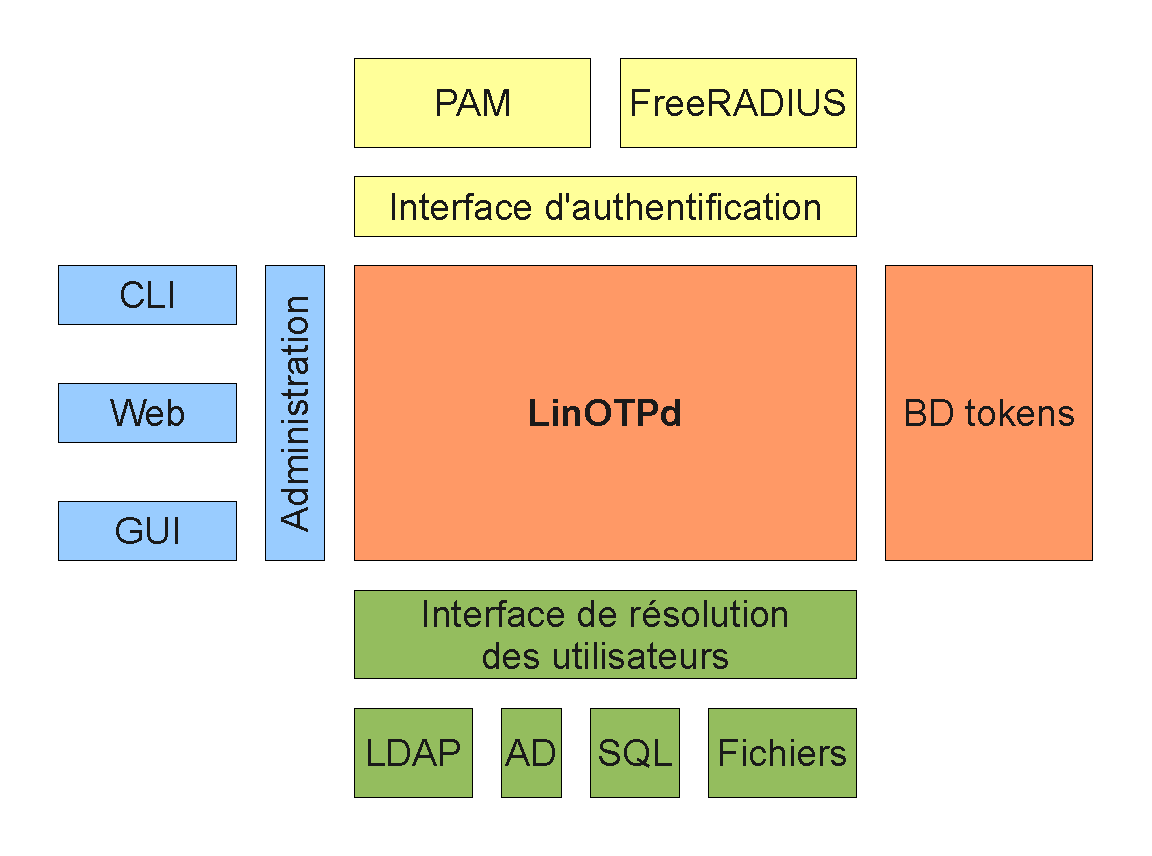
\includegraphics[width=12cm]{linotp/linotp-archi}
	\caption{Architecture modulaire de LinOTP~2}
	\label{figure:linotp:linotp-archi}
\end{figure}


\subsection{Ma démarche}

TODO


\subsection{Architecture mise en place}

TODO

